% Options for packages loaded elsewhere
\PassOptionsToPackage{unicode}{hyperref}
\PassOptionsToPackage{hyphens}{url}
%
\documentclass[
]{article}
\usepackage{amsmath,amssymb}
\usepackage{iftex}
\ifPDFTeX
  \usepackage[T1]{fontenc}
  \usepackage[utf8]{inputenc}
  \usepackage{textcomp} % provide euro and other symbols
\else % if luatex or xetex
  \usepackage{unicode-math} % this also loads fontspec
  \defaultfontfeatures{Scale=MatchLowercase}
  \defaultfontfeatures[\rmfamily]{Ligatures=TeX,Scale=1}
\fi
\usepackage{lmodern}
\ifPDFTeX\else
  % xetex/luatex font selection
\fi
% Use upquote if available, for straight quotes in verbatim environments
\IfFileExists{upquote.sty}{\usepackage{upquote}}{}
\IfFileExists{microtype.sty}{% use microtype if available
  \usepackage[]{microtype}
  \UseMicrotypeSet[protrusion]{basicmath} % disable protrusion for tt fonts
}{}
\makeatletter
\@ifundefined{KOMAClassName}{% if non-KOMA class
  \IfFileExists{parskip.sty}{%
    \usepackage{parskip}
  }{% else
    \setlength{\parindent}{0pt}
    \setlength{\parskip}{6pt plus 2pt minus 1pt}}
}{% if KOMA class
  \KOMAoptions{parskip=half}}
\makeatother
\usepackage{xcolor}
\usepackage[margin=1in]{geometry}
\usepackage{color}
\usepackage{fancyvrb}
\newcommand{\VerbBar}{|}
\newcommand{\VERB}{\Verb[commandchars=\\\{\}]}
\DefineVerbatimEnvironment{Highlighting}{Verbatim}{commandchars=\\\{\}}
% Add ',fontsize=\small' for more characters per line
\usepackage{framed}
\definecolor{shadecolor}{RGB}{248,248,248}
\newenvironment{Shaded}{\begin{snugshade}}{\end{snugshade}}
\newcommand{\AlertTok}[1]{\textcolor[rgb]{0.94,0.16,0.16}{#1}}
\newcommand{\AnnotationTok}[1]{\textcolor[rgb]{0.56,0.35,0.01}{\textbf{\textit{#1}}}}
\newcommand{\AttributeTok}[1]{\textcolor[rgb]{0.13,0.29,0.53}{#1}}
\newcommand{\BaseNTok}[1]{\textcolor[rgb]{0.00,0.00,0.81}{#1}}
\newcommand{\BuiltInTok}[1]{#1}
\newcommand{\CharTok}[1]{\textcolor[rgb]{0.31,0.60,0.02}{#1}}
\newcommand{\CommentTok}[1]{\textcolor[rgb]{0.56,0.35,0.01}{\textit{#1}}}
\newcommand{\CommentVarTok}[1]{\textcolor[rgb]{0.56,0.35,0.01}{\textbf{\textit{#1}}}}
\newcommand{\ConstantTok}[1]{\textcolor[rgb]{0.56,0.35,0.01}{#1}}
\newcommand{\ControlFlowTok}[1]{\textcolor[rgb]{0.13,0.29,0.53}{\textbf{#1}}}
\newcommand{\DataTypeTok}[1]{\textcolor[rgb]{0.13,0.29,0.53}{#1}}
\newcommand{\DecValTok}[1]{\textcolor[rgb]{0.00,0.00,0.81}{#1}}
\newcommand{\DocumentationTok}[1]{\textcolor[rgb]{0.56,0.35,0.01}{\textbf{\textit{#1}}}}
\newcommand{\ErrorTok}[1]{\textcolor[rgb]{0.64,0.00,0.00}{\textbf{#1}}}
\newcommand{\ExtensionTok}[1]{#1}
\newcommand{\FloatTok}[1]{\textcolor[rgb]{0.00,0.00,0.81}{#1}}
\newcommand{\FunctionTok}[1]{\textcolor[rgb]{0.13,0.29,0.53}{\textbf{#1}}}
\newcommand{\ImportTok}[1]{#1}
\newcommand{\InformationTok}[1]{\textcolor[rgb]{0.56,0.35,0.01}{\textbf{\textit{#1}}}}
\newcommand{\KeywordTok}[1]{\textcolor[rgb]{0.13,0.29,0.53}{\textbf{#1}}}
\newcommand{\NormalTok}[1]{#1}
\newcommand{\OperatorTok}[1]{\textcolor[rgb]{0.81,0.36,0.00}{\textbf{#1}}}
\newcommand{\OtherTok}[1]{\textcolor[rgb]{0.56,0.35,0.01}{#1}}
\newcommand{\PreprocessorTok}[1]{\textcolor[rgb]{0.56,0.35,0.01}{\textit{#1}}}
\newcommand{\RegionMarkerTok}[1]{#1}
\newcommand{\SpecialCharTok}[1]{\textcolor[rgb]{0.81,0.36,0.00}{\textbf{#1}}}
\newcommand{\SpecialStringTok}[1]{\textcolor[rgb]{0.31,0.60,0.02}{#1}}
\newcommand{\StringTok}[1]{\textcolor[rgb]{0.31,0.60,0.02}{#1}}
\newcommand{\VariableTok}[1]{\textcolor[rgb]{0.00,0.00,0.00}{#1}}
\newcommand{\VerbatimStringTok}[1]{\textcolor[rgb]{0.31,0.60,0.02}{#1}}
\newcommand{\WarningTok}[1]{\textcolor[rgb]{0.56,0.35,0.01}{\textbf{\textit{#1}}}}
\usepackage{graphicx}
\makeatletter
\def\maxwidth{\ifdim\Gin@nat@width>\linewidth\linewidth\else\Gin@nat@width\fi}
\def\maxheight{\ifdim\Gin@nat@height>\textheight\textheight\else\Gin@nat@height\fi}
\makeatother
% Scale images if necessary, so that they will not overflow the page
% margins by default, and it is still possible to overwrite the defaults
% using explicit options in \includegraphics[width, height, ...]{}
\setkeys{Gin}{width=\maxwidth,height=\maxheight,keepaspectratio}
% Set default figure placement to htbp
\makeatletter
\def\fps@figure{htbp}
\makeatother
\setlength{\emergencystretch}{3em} % prevent overfull lines
\providecommand{\tightlist}{%
  \setlength{\itemsep}{0pt}\setlength{\parskip}{0pt}}
\setcounter{secnumdepth}{5}
\ifLuaTeX
  \usepackage{selnolig}  % disable illegal ligatures
\fi
\IfFileExists{bookmark.sty}{\usepackage{bookmark}}{\usepackage{hyperref}}
\IfFileExists{xurl.sty}{\usepackage{xurl}}{} % add URL line breaks if available
\urlstyle{same}
\hypersetup{
  pdftitle={SC-2 Electric Boogalo},
  pdfauthor={Kieran Morris, Cecina Babich Morrow and Sherman Kjo},
  hidelinks,
  pdfcreator={LaTeX via pandoc}}

\title{SC-2 Electric Boogalo}
\usepackage{etoolbox}
\makeatletter
\providecommand{\subtitle}[1]{% add subtitle to \maketitle
  \apptocmd{\@title}{\par {\large #1 \par}}{}{}
}
\makeatother
\subtitle{Regression on the Irish datset agregated by class}
\author{Kieran Morris, Cecina Babich Morrow and Sherman Kjo}
\date{}

\begin{document}
\maketitle

{
\setcounter{tocdepth}{3}
\tableofcontents
}
\hypertarget{cleaning-the-data}{%
\section{Cleaning the Data}\label{cleaning-the-data}}

\hypertarget{data-overview}{%
\subsection{Data overview}\label{data-overview}}

We are analyzing a set of Irish household electricity demand available
from the \texttt{electBook} package. We have three datasets:

\begin{itemize}
\tightlist
\item
  \texttt{indCons}: 16799 x 2672 matrix of individual household
  electricity consumption. Each column corresponds to a household and
  each row to a time point. Demand is observed every half hour, so there
  are 48 observations per day per household.
\item
  \texttt{survey}: 2672 row dataframe of household survey data. This
  dataset contains household level data on variables such as social
  class, renting vs.~owning, appliances, etc.
\item
  \texttt{extra}: 16799 row dataframe of time-related variables. This
  dataset contains the date-time of each demand observation, time of
  year, day of week, time of day, whether the day was a holiday, and
  external temperature.
\end{itemize}

\begin{Shaded}
\begin{Highlighting}[]
\CommentTok{\# Extract individual dataframes}
\FunctionTok{library}\NormalTok{(electBook)}
\FunctionTok{data}\NormalTok{(Irish)}
\NormalTok{indCons }\OtherTok{\textless{}{-}}\NormalTok{ Irish[[}\StringTok{"indCons"}\NormalTok{]]}
\NormalTok{survey }\OtherTok{\textless{}{-}}\NormalTok{ Irish[[}\StringTok{"survey"}\NormalTok{]]}
\NormalTok{extra }\OtherTok{\textless{}{-}}\NormalTok{ Irish[[}\StringTok{"extra"}\NormalTok{]]}
\end{Highlighting}
\end{Shaded}

\hypertarget{social-class}{%
\subsection{Social class}\label{social-class}}

We wanted to investigate demand patterns across different social
classes. The dataset includes 5 social classes, defined by the
occupation of the head of household:

\begin{itemize}
\tightlist
\item
  AB: managerial roles, administrative or professional
\item
  C1: supervisory, clerical, junior managerial
\item
  C2: skilled manual workers
\item
  DE: semi-skilled and unskilled manual workers, state pensioners,
  casual workers
\item
  F: farmers
\end{itemize}

\begin{Shaded}
\begin{Highlighting}[]
\CommentTok{\# Vector of social classes}
\NormalTok{soc\_classes }\OtherTok{\textless{}{-}} \FunctionTok{c}\NormalTok{(}\FunctionTok{unique}\NormalTok{(survey[}\StringTok{"SOCIALCLASS"}\NormalTok{]))}\SpecialCharTok{$}\NormalTok{SOCIALCLASS}
\end{Highlighting}
\end{Shaded}

** Insert plot of demand patterns for different classes **

We modeled the average demand for each social class separately.

\hypertarget{loading-and-structure}{%
\subsection{Loading and Structure}\label{loading-and-structure}}

We cleaned the data using the code available in
\href{https://github.com/Shermjj/SC-2-Electric-Boogalo/blob/main/data_cleaning.R}{\texttt{data\_cleaning.R}},
which writes out three dataframes: \texttt{df\_halfhr}, \texttt{df\_hr},
and \texttt{df\_day}. These dataframes contain the half-hourly, hourly,
and daily average demand data for each social class, as well as
temperature (also aggregated to the relevant time scale), time of year
(the time of year with 1st January represented as 0 and 31st December
represented as 1), and day of the week. These dataframes are written to
the
\href{https://github.com/Shermjj/SC-2-Electric-Boogalo/tree/main/data}{\texttt{data}
folder}.

\hypertarget{feature-engineering}{%
\subsection{Feature engineering}\label{feature-engineering}}

Based on exploratory data analysis, we created some features from the
dataset to model demand. Feature engineering (with the exception of the
addition of the Fourier terms) was performed in the
\href{https://github.com/Shermjj/SC-2-Electric-Boogalo/blob/main/feature_engineering.R}{\texttt{feature\_engineering.R}
script}, and the resulting dataframes \texttt{df\_halfhr\_scaled},
\texttt{df\_hr\_scaled}, and \texttt{df\_day\_scaled} were saved to the
\href{https://github.com/Shermjj/SC-2-Electric-Boogalo/tree/main/data}{\texttt{data}
folder}.

\begin{Shaded}
\begin{Highlighting}[]
\CommentTok{\# Load transformed data for all time scales}
\NormalTok{df\_halfhr\_scaled }\OtherTok{\textless{}{-}} \FunctionTok{readRDS}\NormalTok{(here}\SpecialCharTok{::}\FunctionTok{here}\NormalTok{(}\StringTok{"data/df\_halfhr\_scaled.RData"}\NormalTok{))}
\NormalTok{df\_hr\_scaled }\OtherTok{\textless{}{-}} \FunctionTok{readRDS}\NormalTok{(here}\SpecialCharTok{::}\FunctionTok{here}\NormalTok{(}\StringTok{"data/df\_hr\_scaled.RData"}\NormalTok{))}
\NormalTok{df\_day\_scaled }\OtherTok{\textless{}{-}} \FunctionTok{readRDS}\NormalTok{(here}\SpecialCharTok{::}\FunctionTok{here}\NormalTok{(}\StringTok{"data/df\_day\_scaled.RData"}\NormalTok{))}
\end{Highlighting}
\end{Shaded}

\hypertarget{time-related-features}{%
\subsubsection{Time-related features}\label{time-related-features}}

We extracted the hour of the day and the month from the date-time
variable. We also included a quadratic term for temperature to capture
the non-linear relationship between temperature and demand. We also used
one-hot encoding to include the day of the week in our models.

\hypertarget{temperature}{%
\subsubsection{Temperature}\label{temperature}}

We can visualize the relationship between temperature and the aggregate
demand over time across all households:

\begin{Shaded}
\begin{Highlighting}[]
\FunctionTok{library}\NormalTok{(tidyverse)}

\CommentTok{\# Aggregate demand over all households}
\NormalTok{agg }\OtherTok{\textless{}{-}} \FunctionTok{rowSums}\NormalTok{(indCons)}
\CommentTok{\# Add temperature data}
\NormalTok{temp\_demand }\OtherTok{\textless{}{-}} \FunctionTok{data.frame}\NormalTok{(}\AttributeTok{demand =}\NormalTok{ agg) }\SpecialCharTok{\%\textgreater{}\%}
  \FunctionTok{bind\_cols}\NormalTok{(Irish[[}\StringTok{"extra"}\NormalTok{]])}

\FunctionTok{ggplot}\NormalTok{(temp\_demand, }\FunctionTok{aes}\NormalTok{(}\AttributeTok{x =}\NormalTok{ dateTime, }\AttributeTok{y =}\NormalTok{ demand, }\AttributeTok{color =}\NormalTok{ temp)) }\SpecialCharTok{+}
  \FunctionTok{geom\_point}\NormalTok{() }\SpecialCharTok{+}
\NormalTok{  viridis}\SpecialCharTok{::}\FunctionTok{scale\_color\_viridis}\NormalTok{(}\AttributeTok{option =} \StringTok{"magma"}\NormalTok{) }\SpecialCharTok{+}
  \FunctionTok{labs}\NormalTok{(}\AttributeTok{x =} \StringTok{"Date"}\NormalTok{, }\AttributeTok{y =} \StringTok{"Total Demand"}\NormalTok{, }\AttributeTok{color =} \StringTok{"Temperature"}\NormalTok{) }\SpecialCharTok{+}
  \FunctionTok{theme\_bw}\NormalTok{()}
\end{Highlighting}
\end{Shaded}

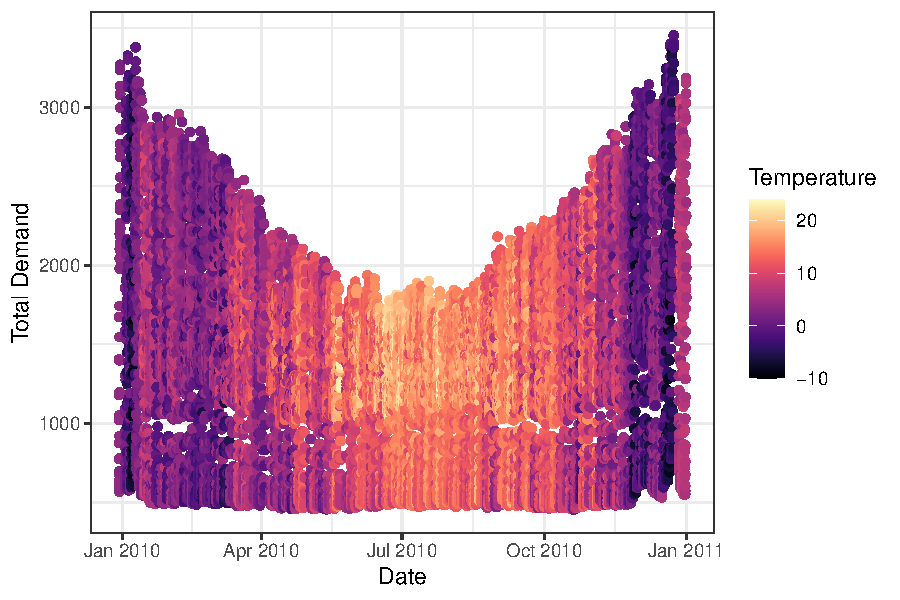
\includegraphics{main_files/figure-latex/unnamed-chunk-4-1.pdf}

We can see that during the warmer summer months, demand dips, although
the pattern is messy. We included linear and quadratic terms for
temperature in our models.

\hypertarget{fourier-terms}{%
\subsubsection{Fourier terms}\label{fourier-terms}}

We used Fourier terms to capture the patterns of seasonality in the
data. Fourier terms are a set of sine and cosine functions with
different frequencies that can be used to model periodic patterns. For a
given period \(P\), the Fourier terms are defined as follows:
\[\text{sin}_k(t) = \sin\left(\frac{2\pi kt}{P}\right), \quad \text{cos}_k(t) = \cos\left(\frac{2\pi kt}{P}\right)\]
where \(k\) is the frequency and \(t\) is the time. Then a partial
Fourier sum can be written as
\[ y(t) = \beta_0 + \sum_{k=1}^{K} \left( \beta_{1k} \sin\left(\frac{2\pi kt}{P}\right) + \beta_{2k} \cos\left(\frac{2\pi kt}{P}\right) \right) \]
where \(K\) is the maximum order of Fourier terms to use.

We used Fourier terms to model the daily and annual seasonality in the
data. Since our dataset is missing data for some days, we needed to
adjust the \(t\) used to calculate the Fourier terms to account for
these gaps. In the
\href{https://github.com/Shermjj/SC-2-Electric-Boogalo/blob/main/feature_engineering.R}{\texttt{feature\_engineering.R}
script}, we added the variable \texttt{counter} to all dataframes. This
variable increments by one for each time step (half hour, hour, or day)
in the dataframe, reflecting the fact that some days are missing. These
\texttt{counter} variables were then used later on to generate Fourier
terms for our models. We wrote an \texttt{Rcpp} function in our package
called \texttt{GenFT}, which creates a matrix of Fourier terms given a
time counter variable representing \(t\), the maximum order of the
Fourier terms \(K\), and the number of time increments in a period
\(P\).

\textbf{Insert example of \texttt{generate\_fourier\_terms} function}

\hypertarget{scaling}{%
\subsection{Scaling}\label{scaling}}

We centered and scaled all variables used in the models.

\hypertarget{training-and-testing}{%
\subsection{Training and testing}\label{training-and-testing}}

Because this is time series data, we needed to make sure the training
and testing data were both contiguous. We trained the models on the
first 90\% of the rows and tested on the final 10\%.

\hypertarget{elecforecast-package}{%
\section{\texorpdfstring{\texttt{ElecForecast}
package}{ElecForecast package}}\label{elecforecast-package}}

\textbf{Insert short description of package, what it does, how to
install it}

\begin{Shaded}
\begin{Highlighting}[]
\CommentTok{\# Load our package}
\FunctionTok{library}\NormalTok{(ElecForecast)}
\end{Highlighting}
\end{Shaded}

\hypertarget{ridge-regression}{%
\section{Ridge Regression}\label{ridge-regression}}

\hypertarget{theory}{%
\subsection{Theory}\label{theory}}

Ridge regression is a method for penalized regression. Consider the
model \[Y_i^0 = \alpha + \beta x_i^0 + \epsilon_i, \quad  i = 1,..., n\]
where \(\beta \in \mathbb{R}^p\), \(\alpha \in \mathbb{R}\), and for all
\(i, l \in \{1, ..., n\}\), \(\mathbb{E}[\epsilon_i] = 0\) and
\(\mathbb{E}[\epsilon_i \epsilon_l] = \sigma^2 \delta_{il}\) for some
\(\sigma^2 > 0\). Then the ridge regression estimator is defined as the
minimizer of the following objective function:
\[(\hat{\alpha}_\lambda, \hat{\beta}_\lambda) = \mathrm{argmin}_{\alpha \in \mathbb{R}, \beta \in \mathbb{R}^p} \lVert y^0 - \alpha - \boldsymbol{X}^0 \beta \rVert^2_2 + \lambda \lVert \beta \rVert^2_2\]
where \(\lambda > 0\) is a tuning parameter and
\(\lVert \cdot \rVert_2\) denotes the Euclidean norm. Ridge regression
is thus imposing a penalty on the size of \(\beta\), with the strength
of that penalty determined by the choice of \(\lambda\). The
coefficients will be shrunk towards zero, but will not be set to zero
(as opposed to in lasso regression).

\hypertarget{model}{%
\subsection{Model}\label{model}}

We performed ridge regression using the model detailed above, with the
following input variables:

\begin{itemize}
\tightlist
\item
  Temperature and squared temperature
\item
  Time of year
\item
  Hour
\item
  Month
\item
  One-hot encoded variables for each day of the week
\item
  Daily Fourier terms
  \(\text{sin}_k(t) = \sin\left(\frac{2\pi kt}{P}\right), \quad \text{cos}_k(t) = \cos\left(\frac{2\pi kt}{P}\right)\)
  for \(k \in \{1,...,K\}\)
\item
  Annual Fourier terms likewise
\end{itemize}

We predicted demand for each of the five social classes at all three
time scales (half hour, hour, and day).

We had two hyperparameters to tune: the standard ridge regression
parameter \(\lambda\) and the maximum order of the Fourier terms
included \(K\). For sake of simplicity, we elected to use the same \(K\)
value for both the daily and the annual terms.

\hypertarget{implementation}{%
\subsection{Implementation}\label{implementation}}

We implemented ridge regression using \texttt{RcppArmadillo} in our
function \texttt{RidgeReg}. We also wrote a function
\texttt{RidgeRegPar} for ridge regression using \texttt{RcppParallel} to
parallelise the matrix multiplication. We can compare the results of
\texttt{RidgeRegPar} with those of the \texttt{glmnet} package:

\begin{Shaded}
\begin{Highlighting}[]
\CommentTok{\# library(glmnet)}
\CommentTok{\# }
\CommentTok{\# \# Example data}
\CommentTok{\# ex\_x \textless{}{-} matrix(rnorm(100 * 20), 100, 20)}
\CommentTok{\# ex\_y \textless{}{-} rnorm(100)}
\CommentTok{\# }
\CommentTok{\# \# Fit ridge regression using glmnet}
\CommentTok{\# fit\_glmnet \textless{}{-} cv.glmnet(ex\_x,}
\CommentTok{\#                         ex\_y,}
\CommentTok{\#                         family = "gaussian",}
\CommentTok{\#                         alpha = 0,}
\CommentTok{\#                         type.measure = "mse",}
\CommentTok{\#                         nfolds = 10)}
\CommentTok{\# ex\_pred\_glmnet \textless{}{-} predict(fit\_glmnet, newx = ex\_x)}
\CommentTok{\# }
\CommentTok{\# \# Fit ridge regression using RidgeRegPar}
\CommentTok{\# fit\_RidgeRegPar \textless{}{-} RidgeRegPar(ex\_x,}
\CommentTok{\#                                ex\_y, }
\CommentTok{\#                                \# Use same lambda as glmnet for comparison}
\CommentTok{\#                                lambda = fit\_glmnet$lambda.1se * nrow(ex\_x)}
\CommentTok{\#                                )}
\CommentTok{\# ex\_pred\_RidgeRegPar \textless{}{-} cbind(1, ex\_x) \%*\% fit\_RidgeRegPar$coefficients}
\CommentTok{\# }
\CommentTok{\# \# Compare predictions}
\CommentTok{\# ex\_df \textless{}{-} data.frame(y = ex\_y,}
\CommentTok{\#                     glmnet\_pred = ex\_pred\_glmnet,}
\CommentTok{\#                     RidgeRegPar\_pred = ex\_pred\_RidgeRegPar)}
\end{Highlighting}
\end{Shaded}

To select \(\lambda\) and \(K\), we used \(k\)-fold cross-validation to
perform a grid search across all combinations of \(\lambda\) and \(K\).
We implemented this cross-validation in the function
\texttt{parallel\_ridge\_cross\_validation}.

\hypertarget{results}{%
\subsection{Results}\label{results}}

\hypertarget{half-hour}{%
\subsubsection{Half hour}\label{half-hour}}

We first split the dataset into training and testing sets:

\begin{Shaded}
\begin{Highlighting}[]
\CommentTok{\# Split the data into training and test sets}
\CommentTok{\# 90\% training set}
\NormalTok{n\_train\_halfhr }\OtherTok{\textless{}{-}} \FunctionTok{round}\NormalTok{(}\FloatTok{0.9}\SpecialCharTok{*}\FunctionTok{nrow}\NormalTok{(df\_halfhr\_scaled))}
\CommentTok{\# Training and testing counter }
\NormalTok{train\_counter\_halfhr }\OtherTok{\textless{}{-}}\NormalTok{ df\_halfhr\_scaled}\SpecialCharTok{$}\NormalTok{counter[}\DecValTok{1}\SpecialCharTok{:}\NormalTok{n\_train\_halfhr]}
\NormalTok{test\_counter\_halfhr }\OtherTok{\textless{}{-}}\NormalTok{ df\_halfhr\_scaled}\SpecialCharTok{$}\NormalTok{counter[}\SpecialCharTok{{-}}\NormalTok{(}\DecValTok{1}\SpecialCharTok{:}\NormalTok{n\_train\_halfhr)]}
\CommentTok{\# Training and testing features}
\NormalTok{halfhr\_features\_train }\OtherTok{\textless{}{-}}\NormalTok{ df\_halfhr\_scaled[}\DecValTok{1}\SpecialCharTok{:}\NormalTok{n\_train\_halfhr,] }\SpecialCharTok{\%\textgreater{}\%} 
  \FunctionTok{select}\NormalTok{(}\SpecialCharTok{{-}}\NormalTok{counter)}
\NormalTok{halfhr\_features\_test }\OtherTok{\textless{}{-}}\NormalTok{ df\_halfhr\_scaled[}\SpecialCharTok{{-}}\NormalTok{(}\DecValTok{1}\SpecialCharTok{:}\NormalTok{n\_train\_halfhr),] }\SpecialCharTok{\%\textgreater{}\%} 
  \FunctionTok{select}\NormalTok{(}\SpecialCharTok{{-}}\NormalTok{counter)}
\end{Highlighting}
\end{Shaded}

Next, we perform 5-fold cross-validation to identify the \(\lambda\) and
\(K\) values that minimize mean squared error. We did this for each of
the five social classes.

\begin{Shaded}
\begin{Highlighting}[]
\CommentTok{\# Range of lambda values}
\NormalTok{lambda\_values }\OtherTok{\textless{}{-}} \FunctionTok{seq}\NormalTok{(}\FloatTok{0.01}\NormalTok{, }\DecValTok{1}\NormalTok{, }\AttributeTok{length.out =} \DecValTok{10}\NormalTok{) }\SpecialCharTok{*} \FunctionTok{nrow}\NormalTok{(halfhr\_features\_train)}

\CommentTok{\# lapply over social classes}
\NormalTok{halfhr\_ridge\_results }\OtherTok{\textless{}{-}} \FunctionTok{lapply}\NormalTok{(soc\_classes, }\ControlFlowTok{function}\NormalTok{(class) \{}
\NormalTok{  y\_class }\OtherTok{\textless{}{-}}\NormalTok{ halfhr\_features\_train[[}\FunctionTok{as.character}\NormalTok{(class)]]}
  \CommentTok{\# Perform cross{-}validation}
\NormalTok{  cv\_results }\OtherTok{\textless{}{-}} \FunctionTok{parallel\_ridge\_cross\_validation}\NormalTok{(}
    \AttributeTok{x\_vars =} \FunctionTok{as.matrix}\NormalTok{(halfhr\_features\_train[,}\DecValTok{7}\SpecialCharTok{:}\FunctionTok{ncol}\NormalTok{(halfhr\_features\_train)]), }
    \AttributeTok{y\_var =}\NormalTok{ y\_class,}
    \AttributeTok{time\_counter =}\NormalTok{ train\_counter\_halfhr, }
    \AttributeTok{daily\_period =} \DecValTok{48}\NormalTok{,}
    \AttributeTok{annual\_period =} \DecValTok{48} \SpecialCharTok{*} \DecValTok{365}\NormalTok{,}
    \AttributeTok{max\_K =} \DecValTok{5}\NormalTok{,}
    \AttributeTok{lambda\_values =}\NormalTok{ lambda\_values,}
    \AttributeTok{n\_folds =} \DecValTok{10}
\NormalTok{  )}
  \FunctionTok{return}\NormalTok{(cv\_results)}
\NormalTok{\})}
\FunctionTok{names}\NormalTok{(halfhr\_ridge\_results) }\OtherTok{\textless{}{-}}\NormalTok{ soc\_classes}

\CommentTok{\# Get predictions for each model on the test set}
\NormalTok{halfhr\_ridge\_preds }\OtherTok{\textless{}{-}} \FunctionTok{lapply}\NormalTok{(halfhr\_ridge\_results, }\ControlFlowTok{function}\NormalTok{(cv\_results) \{}
\NormalTok{  preds }\OtherTok{\textless{}{-}} \FunctionTok{predict\_parallel\_ridge\_cv}\NormalTok{(}\AttributeTok{model =}\NormalTok{ cv\_results,}
                                     \AttributeTok{x\_test =} \FunctionTok{as.matrix}\NormalTok{(halfhr\_features\_test[,}\DecValTok{7}\SpecialCharTok{:}\FunctionTok{ncol}\NormalTok{(halfhr\_features\_test)]),}
                                     \AttributeTok{time\_counter =}\NormalTok{ test\_counter\_halfhr,}
                                     \AttributeTok{daily\_period =} \DecValTok{48}\NormalTok{,}
                                     \AttributeTok{annual\_period =} \DecValTok{48} \SpecialCharTok{*} \DecValTok{365}\NormalTok{)}
  \FunctionTok{return}\NormalTok{(preds)}
\NormalTok{\})}
\FunctionTok{names}\NormalTok{(halfhr\_ridge\_preds) }\OtherTok{\textless{}{-}} \FunctionTok{paste0}\NormalTok{(soc\_classes, }\StringTok{"\_preds"}\NormalTok{)}
\end{Highlighting}
\end{Shaded}

We can now visualize the predictions on the testing set:

\begin{Shaded}
\begin{Highlighting}[]
\FunctionTok{library}\NormalTok{(patchwork)}
\CommentTok{\# Dataframe of true values and predictions on test set}
\NormalTok{halfhr\_test\_true\_preds }\OtherTok{\textless{}{-}}\NormalTok{ halfhr\_features\_test }\SpecialCharTok{\%\textgreater{}\%} 
  \FunctionTok{select}\NormalTok{(dateTime, }\FunctionTok{all\_of}\NormalTok{(soc\_classes)) }\SpecialCharTok{\%\textgreater{}\%} 
  \CommentTok{\# Add predictions}
  \FunctionTok{bind\_cols}\NormalTok{(}\FunctionTok{as.data.frame}\NormalTok{(halfhr\_ridge\_preds))}

\CommentTok{\# Plot the predictions for each social class}
\CommentTok{\# Arrange in a grid}
\NormalTok{halfhr\_ridge\_plots }\OtherTok{\textless{}{-}} \FunctionTok{list}\NormalTok{()}
\ControlFlowTok{for}\NormalTok{ (class }\ControlFlowTok{in} \FunctionTok{as.character}\NormalTok{(soc\_classes)) \{}
\NormalTok{  plot\_title }\OtherTok{\textless{}{-}} \FunctionTok{paste}\NormalTok{(}\StringTok{"Half{-}hourly demand predictions for"}\NormalTok{, class)}
\NormalTok{  p }\OtherTok{\textless{}{-}} \FunctionTok{ggplot}\NormalTok{(halfhr\_test\_true\_preds, }\FunctionTok{aes}\NormalTok{(}\AttributeTok{x =}\NormalTok{ dateTime)) }\SpecialCharTok{+}
    \FunctionTok{geom\_line}\NormalTok{(}\FunctionTok{aes}\NormalTok{(}\AttributeTok{y =}\NormalTok{ .data[[class]]), }\AttributeTok{color =} \StringTok{"\#414141"}\NormalTok{) }\SpecialCharTok{+}
    \FunctionTok{geom\_line}\NormalTok{(}\FunctionTok{aes}\NormalTok{(}\AttributeTok{y =}\NormalTok{ .data[[}\FunctionTok{paste0}\NormalTok{(class, }\StringTok{"\_preds"}\NormalTok{)]]), }\AttributeTok{color =} \StringTok{"red"}\NormalTok{) }\SpecialCharTok{+}
    \FunctionTok{labs}\NormalTok{(}\AttributeTok{title =}\NormalTok{ plot\_title, }\AttributeTok{x =} \StringTok{"Date"}\NormalTok{, }\AttributeTok{y =} \StringTok{"Demand"}\NormalTok{) }\SpecialCharTok{+}
    \FunctionTok{theme\_bw}\NormalTok{()}
\NormalTok{  halfhr\_ridge\_plots[[class]] }\OtherTok{\textless{}{-}}\NormalTok{ p}
\NormalTok{\}}
\NormalTok{combined\_halfhr\_ridge\_plot }\OtherTok{\textless{}{-}} \FunctionTok{wrap\_plots}\NormalTok{(halfhr\_ridge\_plots, }\AttributeTok{ncol =} \DecValTok{2}\NormalTok{)}
\NormalTok{combined\_halfhr\_ridge\_plot}
\end{Highlighting}
\end{Shaded}

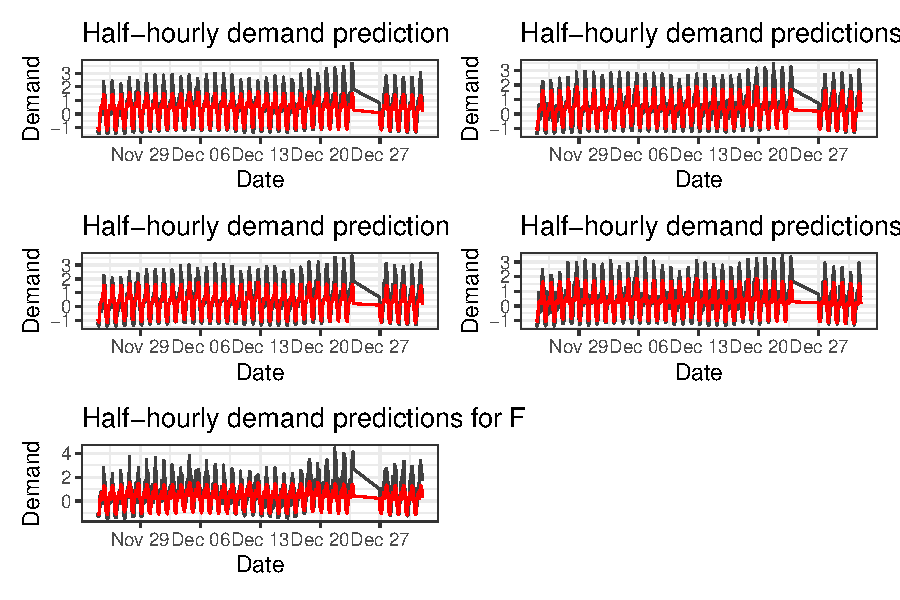
\includegraphics{main_files/figure-latex/unnamed-chunk-9-1.pdf}

\hypertarget{hour}{%
\subsubsection{Hour}\label{hour}}

Split the dataset into training and testing sets:

\begin{Shaded}
\begin{Highlighting}[]
\CommentTok{\# Split the data into training and test sets}
\CommentTok{\# 90\% training set}
\NormalTok{n\_train\_hr }\OtherTok{\textless{}{-}} \FunctionTok{round}\NormalTok{(}\FloatTok{0.9}\SpecialCharTok{*}\FunctionTok{nrow}\NormalTok{(df\_hr\_scaled))}
\NormalTok{hr\_features\_train }\OtherTok{\textless{}{-}}\NormalTok{ df\_hr\_scaled[}\DecValTok{1}\SpecialCharTok{:}\NormalTok{n\_train\_hr,]}
\NormalTok{train\_counter\_hr }\OtherTok{\textless{}{-}}\NormalTok{ df\_hr\_scaled}\SpecialCharTok{$}\NormalTok{counter[}\DecValTok{1}\SpecialCharTok{:}\NormalTok{n\_train\_hr]}
\NormalTok{hr\_features\_test }\OtherTok{\textless{}{-}}\NormalTok{ df\_hr\_scaled[}\SpecialCharTok{{-}}\NormalTok{(}\DecValTok{1}\SpecialCharTok{:}\NormalTok{n\_train\_hr),]}
\NormalTok{test\_counter\_hr }\OtherTok{\textless{}{-}}\NormalTok{ df\_hr\_scaled}\SpecialCharTok{$}\NormalTok{counter[}\SpecialCharTok{{-}}\NormalTok{(}\DecValTok{1}\SpecialCharTok{:}\NormalTok{n\_train\_hr)]}
\end{Highlighting}
\end{Shaded}

\hypertarget{day}{%
\subsubsection{Day}\label{day}}

Split the dataset into training and testing sets:

\begin{Shaded}
\begin{Highlighting}[]
\CommentTok{\# Split the data into training and test sets}
\CommentTok{\# 90\% training set}
\NormalTok{n\_train\_day }\OtherTok{\textless{}{-}} \FunctionTok{round}\NormalTok{(}\FloatTok{0.9}\SpecialCharTok{*}\FunctionTok{nrow}\NormalTok{(df\_day\_scaled))}
\NormalTok{day\_features\_train }\OtherTok{\textless{}{-}}\NormalTok{ df\_day\_scaled[}\DecValTok{1}\SpecialCharTok{:}\NormalTok{n\_train\_day,]}
\NormalTok{train\_counter\_day }\OtherTok{\textless{}{-}}\NormalTok{ df\_day\_scaled}\SpecialCharTok{$}\NormalTok{counter[}\DecValTok{1}\SpecialCharTok{:}\NormalTok{n\_train\_day]}
\NormalTok{day\_features\_test }\OtherTok{\textless{}{-}}\NormalTok{ df\_day\_scaled[}\SpecialCharTok{{-}}\NormalTok{(}\DecValTok{1}\SpecialCharTok{:}\NormalTok{n\_train\_day),]}
\NormalTok{test\_counter\_day }\OtherTok{\textless{}{-}}\NormalTok{ df\_day\_scaled}\SpecialCharTok{$}\NormalTok{counter[}\SpecialCharTok{{-}}\NormalTok{(}\DecValTok{1}\SpecialCharTok{:}\NormalTok{n\_train\_day)]}
\end{Highlighting}
\end{Shaded}

\hypertarget{gaussian-process-regression}{%
\section{Gaussian Process
Regression}\label{gaussian-process-regression}}

\hypertarget{theory-1}{%
\subsection{Theory}\label{theory-1}}

A gaussian process \(W = (W(x))_{x \in \mathcal{X}}\) is a collection of
random variables, which have a joint Gaussian distribution. One useful
fact is that a Gaussian process is completely specified by its mean
(\(\mu:\mathcal{X} \rightarrow \mathbb{R}\)) and covariance
(\(k:\mathcal{X}^2 \rightarrow \mathbb{R}\)) functions - meaning the
objective of GPR is to obtain the mean and covariance. This allows us to
express any finite collection of \(W\) as follows:

\[
(W(x_1), W(x_2), ..., W(x_n)) \sim N((\mu(x_1),...\mu(x_n)), (k(x_i,x_j))_{ij})
\]

We build the following model:

Let \(y_i = f(x_i) + \varepsilon_i\), where
\(\varepsilon_i \sim N(0, \sigma^2)\) and we let \(f\) be a gaussian
process. It can be shown that

\[
f \mid y^0 \sim \text{GP}(f_n,k_n)
\]

where \[f_n(x) = k^n(x)^T(K + \sigma^2I_n)^{-1}y^0,\]
\[k(x,x*) = k(x, x^*) - k^n(x)^T (K + \sigma^2 I_n)^{-1} k^n(x^*)\] and

\[
K = (k(x_i^0,x_j^0))_{ij}
\]

\[
k^n(x) = (k(x_1^0,x),k(x_n^0,x)).
\] Although if it looks scary just remember a computer can do it! This
gives us a way to then model

\[Y^0 \sim \text{N}(0,K _ \lambda I_n),\]

to simulate our results.

In practice, to find the posterior distribution, we maximise the
marginal log-likelihood.

\hypertarget{tuning-hyperparameters}{%
\subsection{Tuning hyperparameters}\label{tuning-hyperparameters}}

For our needs we will use a radial basis function kernel, which has a
single hyperparemter \(l\), often called the bandwidth.

\[
k(x, x') = \exp\left(-\frac{\lVert x - x' \rVert^2}{2l}\right)
\]

We also have the hyperparameter \(\sigma\) which is the standard
deviation of our noise. In order to find the ideal hyperparameters we
will attempt to maximize the marginal log likelihood. The marginal log
likelihood is given by:

\[
\log p(y^0 \mid x^0, l,\sigma^2) = -\frac{1}{2} y^0 (K + \sigma^2 I_n)^{-1} y^0 - \frac{1}{2} \log \lvert K + \sigma^2 I_n \rvert 
\]

where we remove a constant which is irrelevant to the optimisation.
Since this is computationaly intense, we outsource the optimisation to
C++, and integrate it via RcppArmadillo. Below is the C++ code we used,
which can also be found \texttt{gauss\_process\_reg.cpp}:

\begin{Shaded}
\begin{Highlighting}[]
\PreprocessorTok{\#include }\ImportTok{\textless{}RcppArmadillo.h\textgreater{}}
\PreprocessorTok{\#include }\ImportTok{\textless{}optim.hpp\textgreater{}}

\CommentTok{// [[Rcpp::depends(RcppArmadillo)]]}

\CommentTok{// Define the RBF kernel}
\NormalTok{arma}\OperatorTok{::}\NormalTok{mat rbf\_kernel}\OperatorTok{(}\AttributeTok{const}\NormalTok{ arma}\OperatorTok{::}\NormalTok{mat}\OperatorTok{\&}\NormalTok{ X}\OperatorTok{,} \DataTypeTok{double}\NormalTok{ l}\OperatorTok{,} \DataTypeTok{double}\NormalTok{ sigma}\OperatorTok{)} \OperatorTok{\{}
\NormalTok{    arma}\OperatorTok{::}\NormalTok{mat K }\OperatorTok{=}\NormalTok{ arma}\OperatorTok{::}\NormalTok{zeros}\OperatorTok{(}\NormalTok{X}\OperatorTok{.}\NormalTok{n\_rows}\OperatorTok{,}\NormalTok{ X}\OperatorTok{.}\NormalTok{n\_rows}\OperatorTok{);}
    \ControlFlowTok{for} \OperatorTok{(}\DataTypeTok{unsigned}\NormalTok{ i }\OperatorTok{=} \DecValTok{0}\OperatorTok{;}\NormalTok{ i }\OperatorTok{\textless{}}\NormalTok{ X}\OperatorTok{.}\NormalTok{n\_rows}\OperatorTok{;} \OperatorTok{++}\NormalTok{i}\OperatorTok{)} \OperatorTok{\{}
        \ControlFlowTok{for} \OperatorTok{(}\DataTypeTok{unsigned}\NormalTok{ j }\OperatorTok{=} \DecValTok{0}\OperatorTok{;}\NormalTok{ j }\OperatorTok{\textless{}}\NormalTok{ X}\OperatorTok{.}\NormalTok{n\_rows}\OperatorTok{;} \OperatorTok{++}\NormalTok{j}\OperatorTok{)} \OperatorTok{\{}
            \DataTypeTok{double}\NormalTok{ dist }\OperatorTok{=}\NormalTok{ arma}\OperatorTok{::}\NormalTok{norm}\OperatorTok{(}\NormalTok{X}\OperatorTok{.}\NormalTok{row}\OperatorTok{(}\NormalTok{i}\OperatorTok{)} \OperatorTok{{-}}\NormalTok{ X}\OperatorTok{.}\NormalTok{row}\OperatorTok{(}\NormalTok{j}\OperatorTok{),} \DecValTok{2}\OperatorTok{);}
\NormalTok{            K}\OperatorTok{(}\NormalTok{i}\OperatorTok{,}\NormalTok{ j}\OperatorTok{)} \OperatorTok{=} \BuiltInTok{std::}\NormalTok{pow}\OperatorTok{(}\NormalTok{sigma}\OperatorTok{,} \DecValTok{2}\OperatorTok{)} \OperatorTok{*} \BuiltInTok{std::}\NormalTok{exp}\OperatorTok{({-}}\BuiltInTok{std::}\NormalTok{pow}\OperatorTok{(}\NormalTok{dist}\OperatorTok{,} \DecValTok{2}\OperatorTok{)} \OperatorTok{/} \OperatorTok{(}\DecValTok{2} \OperatorTok{*} \BuiltInTok{std::}\NormalTok{pow}\OperatorTok{(}\NormalTok{l}\OperatorTok{,} \DecValTok{2}\OperatorTok{)));}
        \OperatorTok{\}}
    \OperatorTok{\}}
    \ControlFlowTok{return}\NormalTok{ K}\OperatorTok{;}
\OperatorTok{\}}

\CommentTok{// Define the negative log marginal likelihood}
\DataTypeTok{double}\NormalTok{ neg\_log\_marginal\_likelihood}\OperatorTok{(}\AttributeTok{const}\NormalTok{ arma}\OperatorTok{::}\NormalTok{vec}\OperatorTok{\&}\NormalTok{ theta}\OperatorTok{,}\NormalTok{ arma}\OperatorTok{::}\NormalTok{vec}\OperatorTok{*}\NormalTok{ grad\_out}\OperatorTok{,} \DataTypeTok{void}\OperatorTok{*}\NormalTok{ opt\_data}\OperatorTok{)} \OperatorTok{\{}
    \CommentTok{// Extract data and parameters}
\NormalTok{    arma}\OperatorTok{::}\NormalTok{mat X }\OperatorTok{=} \OperatorTok{*}\KeywordTok{static\_cast}\OperatorTok{\textless{}}\NormalTok{arma}\OperatorTok{::}\NormalTok{mat}\OperatorTok{*\textgreater{}(}\NormalTok{opt\_data}\OperatorTok{);}
\NormalTok{    arma}\OperatorTok{::}\NormalTok{vec y }\OperatorTok{=} \OperatorTok{*}\KeywordTok{static\_cast}\OperatorTok{\textless{}}\NormalTok{arma}\OperatorTok{::}\NormalTok{vec}\OperatorTok{*\textgreater{}(}\NormalTok{opt\_data}\OperatorTok{);}
    \DataTypeTok{double}\NormalTok{ l }\OperatorTok{=}\NormalTok{ theta}\OperatorTok{(}\DecValTok{0}\OperatorTok{);}
    \DataTypeTok{double}\NormalTok{ sigma }\OperatorTok{=}\NormalTok{ theta}\OperatorTok{(}\DecValTok{1}\OperatorTok{);}

    \CommentTok{// Calculate the kernel matrix}
\NormalTok{    arma}\OperatorTok{::}\NormalTok{mat K }\OperatorTok{=}\NormalTok{ rbf\_kernel}\OperatorTok{(}\NormalTok{X}\OperatorTok{,}\NormalTok{ l}\OperatorTok{,}\NormalTok{ sigma}\OperatorTok{);}

    \CommentTok{// Calculate the log marginal likelihood}
    
    \DataTypeTok{double}\NormalTok{ log\_likelihood }\OperatorTok{=} \OperatorTok{{-}}\FloatTok{0.5} \OperatorTok{*}\NormalTok{ arma}\OperatorTok{::}\NormalTok{as\_scalar}\OperatorTok{(}\NormalTok{y}\OperatorTok{.}\NormalTok{t}\OperatorTok{()} \OperatorTok{*}\NormalTok{ arma}\OperatorTok{::}\NormalTok{solve}\OperatorTok{(}\NormalTok{K}\OperatorTok{,}\NormalTok{ y}\OperatorTok{))} \OperatorTok{{-}} \FloatTok{0.5} \OperatorTok{*}\NormalTok{ arma}\OperatorTok{::}\NormalTok{log\_det}\OperatorTok{(}\NormalTok{K }\OperatorTok{+}\NormalTok{ l }\OperatorTok{)} \OperatorTok{{-}} \FloatTok{0.5} \OperatorTok{*}\NormalTok{ X}\OperatorTok{.}\NormalTok{n\_rows }\OperatorTok{*} \BuiltInTok{std::}\NormalTok{log}\OperatorTok{(}\DecValTok{2} \OperatorTok{*}\NormalTok{ M\_PI}\OperatorTok{);}

    \CommentTok{// Return the negative log marginal likelihood}
    \ControlFlowTok{return} \OperatorTok{{-}}\NormalTok{log\_likelihood}\OperatorTok{;}
\OperatorTok{\}}

\CommentTok{// [[Rcpp::export]]}
\NormalTok{arma}\OperatorTok{::}\NormalTok{vec optimise\_gaussian\_process}\OperatorTok{(}\NormalTok{arma}\OperatorTok{::}\NormalTok{mat X}\OperatorTok{,}\NormalTok{ arma}\OperatorTok{::}\NormalTok{vec y}\OperatorTok{)} \OperatorTok{\{}
    \CommentTok{// Initial guess for the parameters}
\NormalTok{    arma}\OperatorTok{::}\NormalTok{vec theta }\OperatorTok{=}\NormalTok{ arma}\OperatorTok{::}\NormalTok{ones}\OperatorTok{(}\DecValTok{2}\OperatorTok{);}

    \CommentTok{// Optimise the negative log marginal likelihood}
    \DataTypeTok{bool}\NormalTok{ success }\OperatorTok{=}\NormalTok{ optim}\OperatorTok{::}\NormalTok{de}\OperatorTok{(}\NormalTok{theta}\OperatorTok{,}\NormalTok{ neg\_log\_marginal\_likelihood}\OperatorTok{,} \OperatorTok{\&}\NormalTok{X}\OperatorTok{);}

    \CommentTok{// Return the optimised parameters}
    \ControlFlowTok{return}\NormalTok{ theta}\OperatorTok{;}
\OperatorTok{\}}
\end{Highlighting}
\end{Shaded}

We parallize over the grid of initial choices to speed up the
optimisation. As we going to be performing this on different sized
datasets (half hourly, hourly and daily) it is unwise to perform
parallisation over those. Instead we created an wrapper function in
\texttt{R} which can take in an arbitrary dataset. We display it below
but it can be found in \texttt{gauss\_process\_reg.R}:

\begin{Shaded}
\begin{Highlighting}[]
\NormalTok{find\_optimal\_params }\OtherTok{\textless{}{-}} \ControlFlowTok{function}\NormalTok{(X, y) \{}
  \CommentTok{\# Source the C++ file}
  \FunctionTok{sourceCpp}\NormalTok{(}\StringTok{"gauss\_process\_reg.cpp"}\NormalTok{)}
  
  \CommentTok{\# Call the C++ function}
\NormalTok{  theta }\OtherTok{\textless{}{-}} \FunctionTok{optimise\_gaussian\_process}\NormalTok{(X, y)}
  
  \CommentTok{\# Return the optimal parameters}
  \FunctionTok{return}\NormalTok{(theta)}
\NormalTok{\}}
\end{Highlighting}
\end{Shaded}

\hypertarget{implementation-1}{%
\subsection{Implementation}\label{implementation-1}}

For the gaussian process regression, we will use the
\texttt{kernlab::gausspr} function, which can perform multivariate
gaussian process regression, allowing us to add our additional features
as covariates. Since we have our ideal hyperparameters \(l\) and
\(\sigma\) for each dataset, we can now fit the gaussian process
regression model fairly easily. Source code for the following can be
found in \texttt{gauss\_process\_reg.R}:

\begin{Shaded}
\begin{Highlighting}[]
\NormalTok{gaussian\_process\_reg }\OtherTok{\textless{}{-}} \ControlFlowTok{function}\NormalTok{(data,}
                                 \AttributeTok{class =} \StringTok{"DE"}\NormalTok{,}
                                 \AttributeTok{kernel =} \StringTok{"rbfdot"}\NormalTok{,}
                                 \AttributeTok{plot =} \ConstantTok{FALSE}\NormalTok{,}
                                 \AttributeTok{sigma =} \DecValTok{100}\NormalTok{) \{}

  \CommentTok{\#Training and test set, first 90\% of data is training, last 10\% is test}
\NormalTok{  train\_index }\OtherTok{\textless{}{-}} \FunctionTok{round}\NormalTok{(}\FunctionTok{nrow}\NormalTok{(data) }\SpecialCharTok{*} \FloatTok{0.9}\NormalTok{)}
\NormalTok{  train\_set }\OtherTok{\textless{}{-}}\NormalTok{ data[}\DecValTok{1}\SpecialCharTok{:}\NormalTok{train\_index, ]}
\NormalTok{  test\_set }\OtherTok{\textless{}{-}}\NormalTok{ data[(train\_index }\SpecialCharTok{+} \DecValTok{1}\NormalTok{)}\SpecialCharTok{:}\FunctionTok{nrow}\NormalTok{(data), ]}

  \CommentTok{\# Define the Gaussian process model}
\NormalTok{  gpr\_model }\OtherTok{\textless{}{-}}\NormalTok{ kernlab}\SpecialCharTok{::}\FunctionTok{gausspr}\NormalTok{(}\FunctionTok{as.matrix}\NormalTok{(train\_set[, }\FunctionTok{c}\NormalTok{(}\StringTok{"toy"}\NormalTok{, }\StringTok{"temp"}\NormalTok{)]),}
                                \FunctionTok{as.vector}\NormalTok{(train\_set[[class]]),}
                                \AttributeTok{kernel =}\NormalTok{ kernel, }\AttributeTok{kpar =} \FunctionTok{list}\NormalTok{(}\AttributeTok{sigma =}\NormalTok{ sigma))}

  \CommentTok{\# Predict the mean function for plotting}
\NormalTok{  mean\_func }\OtherTok{\textless{}{-}} \FunctionTok{predict}\NormalTok{(gpr\_model, }\FunctionTok{as.vector}\NormalTok{(data}\SpecialCharTok{$}\NormalTok{toy))}
\NormalTok{  prediction }\OtherTok{\textless{}{-}} \FunctionTok{data.frame}\NormalTok{(}
                           \AttributeTok{toy =}\NormalTok{ data}\SpecialCharTok{$}\NormalTok{toy,}
                           \AttributeTok{mean =}\NormalTok{ mean\_func)}

\NormalTok{  data\_with\_pred }\OtherTok{\textless{}{-}} \FunctionTok{left\_join}\NormalTok{(data, prediction, }\AttributeTok{by =} \StringTok{"toy"}\NormalTok{)}

  \CommentTok{\# Evaluate performance}
\NormalTok{  test\_mean\_func }\OtherTok{\textless{}{-}} \FunctionTok{predict}\NormalTok{(gpr\_model, }\FunctionTok{as.vector}\NormalTok{(test\_set}\SpecialCharTok{$}\NormalTok{toy))}
\NormalTok{  performance }\OtherTok{\textless{}{-}} \FunctionTok{postResample}\NormalTok{(}\AttributeTok{pred =}\NormalTok{ test\_mean\_func, }\AttributeTok{obs =}\NormalTok{ test\_set}\SpecialCharTok{$}\NormalTok{DE)}

  \CommentTok{\# Include Plots ?}
  \ControlFlowTok{if}\NormalTok{ (plot)\{}
\NormalTok{    pl }\OtherTok{\textless{}{-}} \FunctionTok{ggplot}\NormalTok{(data\_with\_pred, }\FunctionTok{aes}\NormalTok{(}\AttributeTok{x =}\NormalTok{ toy)) }\SpecialCharTok{+}
      \FunctionTok{geom\_point}\NormalTok{(}\FunctionTok{aes}\NormalTok{(}\AttributeTok{y =} \FunctionTok{get}\NormalTok{(class)), }\AttributeTok{color =} \StringTok{"\#414141"}\NormalTok{) }\SpecialCharTok{+}
      \FunctionTok{geom\_line}\NormalTok{(}\FunctionTok{aes}\NormalTok{(}\AttributeTok{y =}\NormalTok{ mean), }\AttributeTok{color =}\NormalTok{ class\_colours[class]) }\SpecialCharTok{+}
      \FunctionTok{labs}\NormalTok{(}\AttributeTok{title =} \StringTok{"GPR model predictions"}\NormalTok{,}
           \AttributeTok{x =} \StringTok{"Date"}\NormalTok{, }\AttributeTok{y =} \StringTok{"Demand"}\NormalTok{)}
\NormalTok{    pl}
\NormalTok{  \} }\ControlFlowTok{else}\NormalTok{ \{}
\NormalTok{    pl }\OtherTok{\textless{}{-}} \ConstantTok{NULL}
\NormalTok{  \}}
  \FunctionTok{return}\NormalTok{(}\FunctionTok{list}\NormalTok{(}\AttributeTok{model =}\NormalTok{ gpr\_model,}
\NormalTok{              data }\OtherTok{\textless{}{-}}\NormalTok{ data\_with\_pred,}
\NormalTok{              performance,}
              \AttributeTok{plot =}\NormalTok{ pl))}
\NormalTok{\}}
\end{Highlighting}
\end{Shaded}

\hypertarget{results-1}{%
\section{Results}\label{results-1}}

\end{document}
